% Options for packages loaded elsewhere
\PassOptionsToPackage{unicode}{hyperref}
\PassOptionsToPackage{hyphens}{url}
%
\documentclass[
]{article}
\usepackage{amsmath,amssymb}
\usepackage{lmodern}
\usepackage{iftex}
\ifPDFTeX
  \usepackage[T1]{fontenc}
  \usepackage[utf8]{inputenc}
  \usepackage{textcomp} % provide euro and other symbols
\else % if luatex or xetex
  \usepackage{unicode-math}
  \defaultfontfeatures{Scale=MatchLowercase}
  \defaultfontfeatures[\rmfamily]{Ligatures=TeX,Scale=1}
\fi
% Use upquote if available, for straight quotes in verbatim environments
\IfFileExists{upquote.sty}{\usepackage{upquote}}{}
\IfFileExists{microtype.sty}{% use microtype if available
  \usepackage[]{microtype}
  \UseMicrotypeSet[protrusion]{basicmath} % disable protrusion for tt fonts
}{}
\makeatletter
\@ifundefined{KOMAClassName}{% if non-KOMA class
  \IfFileExists{parskip.sty}{%
    \usepackage{parskip}
  }{% else
    \setlength{\parindent}{0pt}
    \setlength{\parskip}{6pt plus 2pt minus 1pt}}
}{% if KOMA class
  \KOMAoptions{parskip=half}}
\makeatother
\usepackage{xcolor}
\usepackage[margin=1in]{geometry}
\usepackage{graphicx}
\makeatletter
\def\maxwidth{\ifdim\Gin@nat@width>\linewidth\linewidth\else\Gin@nat@width\fi}
\def\maxheight{\ifdim\Gin@nat@height>\textheight\textheight\else\Gin@nat@height\fi}
\makeatother
% Scale images if necessary, so that they will not overflow the page
% margins by default, and it is still possible to overwrite the defaults
% using explicit options in \includegraphics[width, height, ...]{}
\setkeys{Gin}{width=\maxwidth,height=\maxheight,keepaspectratio}
% Set default figure placement to htbp
\makeatletter
\def\fps@figure{htbp}
\makeatother
\setlength{\emergencystretch}{3em} % prevent overfull lines
\providecommand{\tightlist}{%
  \setlength{\itemsep}{0pt}\setlength{\parskip}{0pt}}
\setcounter{secnumdepth}{-\maxdimen} % remove section numbering
\usepackage{booktabs}
\usepackage{siunitx}

  \newcolumntype{d}{S[
    input-open-uncertainty=,
    input-close-uncertainty=,
    parse-numbers = false,
    table-align-text-pre=false,
    table-align-text-post=false
  ]}
  
\usepackage{longtable}
\usepackage{array}
\usepackage{multirow}
\usepackage{wrapfig}
\usepackage{float}
\usepackage{colortbl}
\usepackage{pdflscape}
\usepackage{tabu}
\usepackage{threeparttable}
\usepackage{threeparttablex}
\usepackage[normalem]{ulem}
\usepackage{makecell}
\usepackage{xcolor}
\ifLuaTeX
  \usepackage{selnolig}  % disable illegal ligatures
\fi
\IfFileExists{bookmark.sty}{\usepackage{bookmark}}{\usepackage{hyperref}}
\IfFileExists{xurl.sty}{\usepackage{xurl}}{} % add URL line breaks if available
\urlstyle{same} % disable monospaced font for URLs
\hypersetup{
  pdftitle={ReplicacionAbortion},
  pdfauthor={Jaquelin Morillo},
  hidelinks,
  pdfcreator={LaTeX via pandoc}}

\title{ReplicacionAbortion}
\author{Jaquelin Morillo}
\date{2022-12-19}

\begin{document}
\maketitle

\hypertarget{replicaciuxf3n-abortion-legalization-and-long-term-gonorrhea-incidence}{%
\subsubsection{1. Replicación Abortion legalization and long-term
gonorrhea
incidence}\label{replicaciuxf3n-abortion-legalization-and-long-term-gonorrhea-incidence}}

\url{https://mixtape.scunning.com/09-difference_in_differences\#abortion-legalization-and-long-term-gonorrhea-incidence}

\emph{Github:}
\url{https://github.com/JaquelinMorillo/ReplicacionAbortion}

\#1
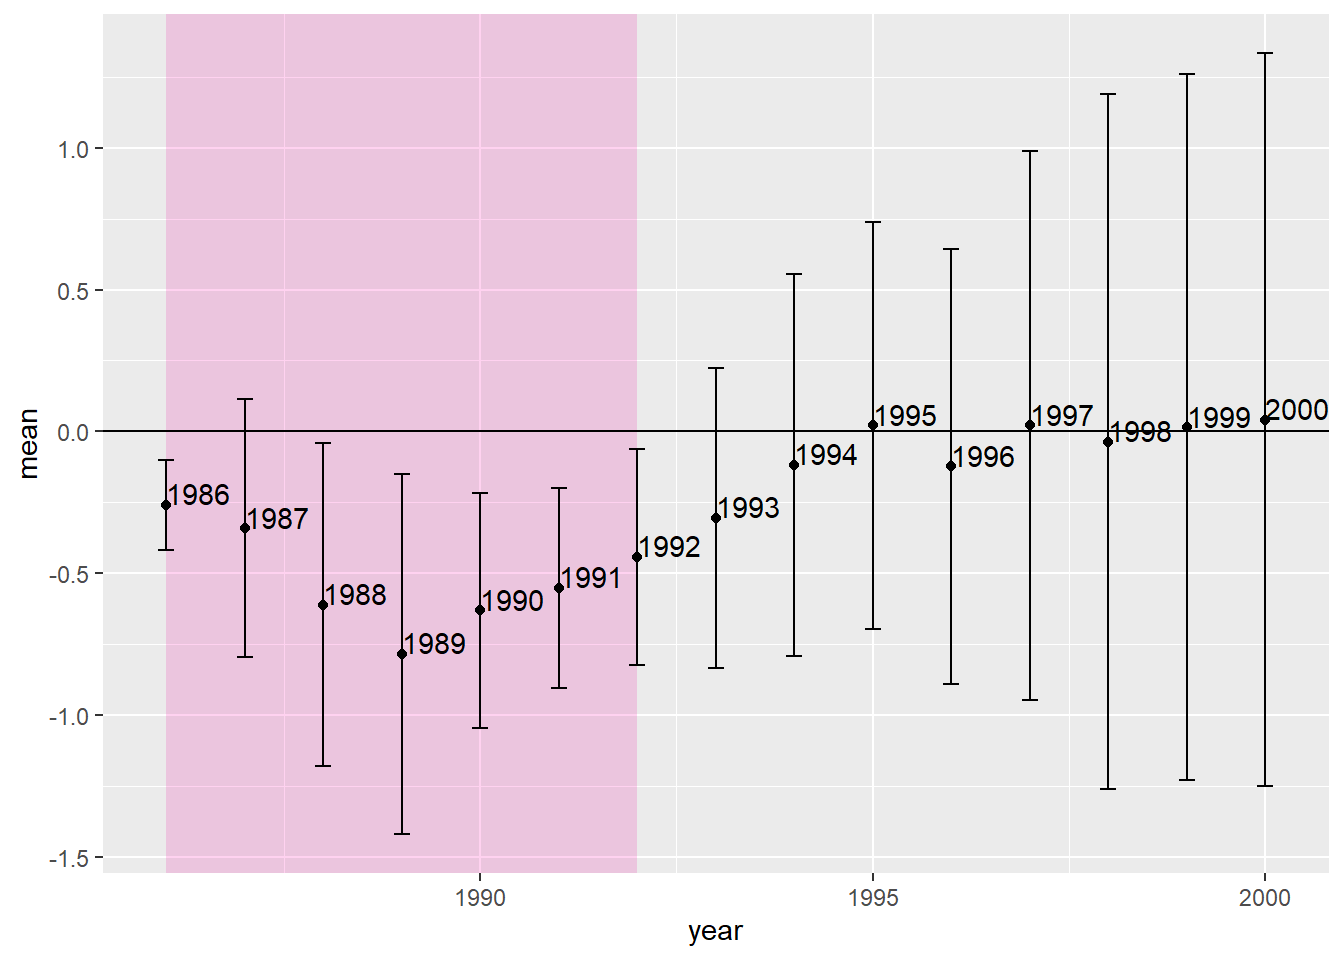
\includegraphics{ReplicacionAbortion_files/figure-latex/unnamed-chunk-1-1.pdf}

\#2
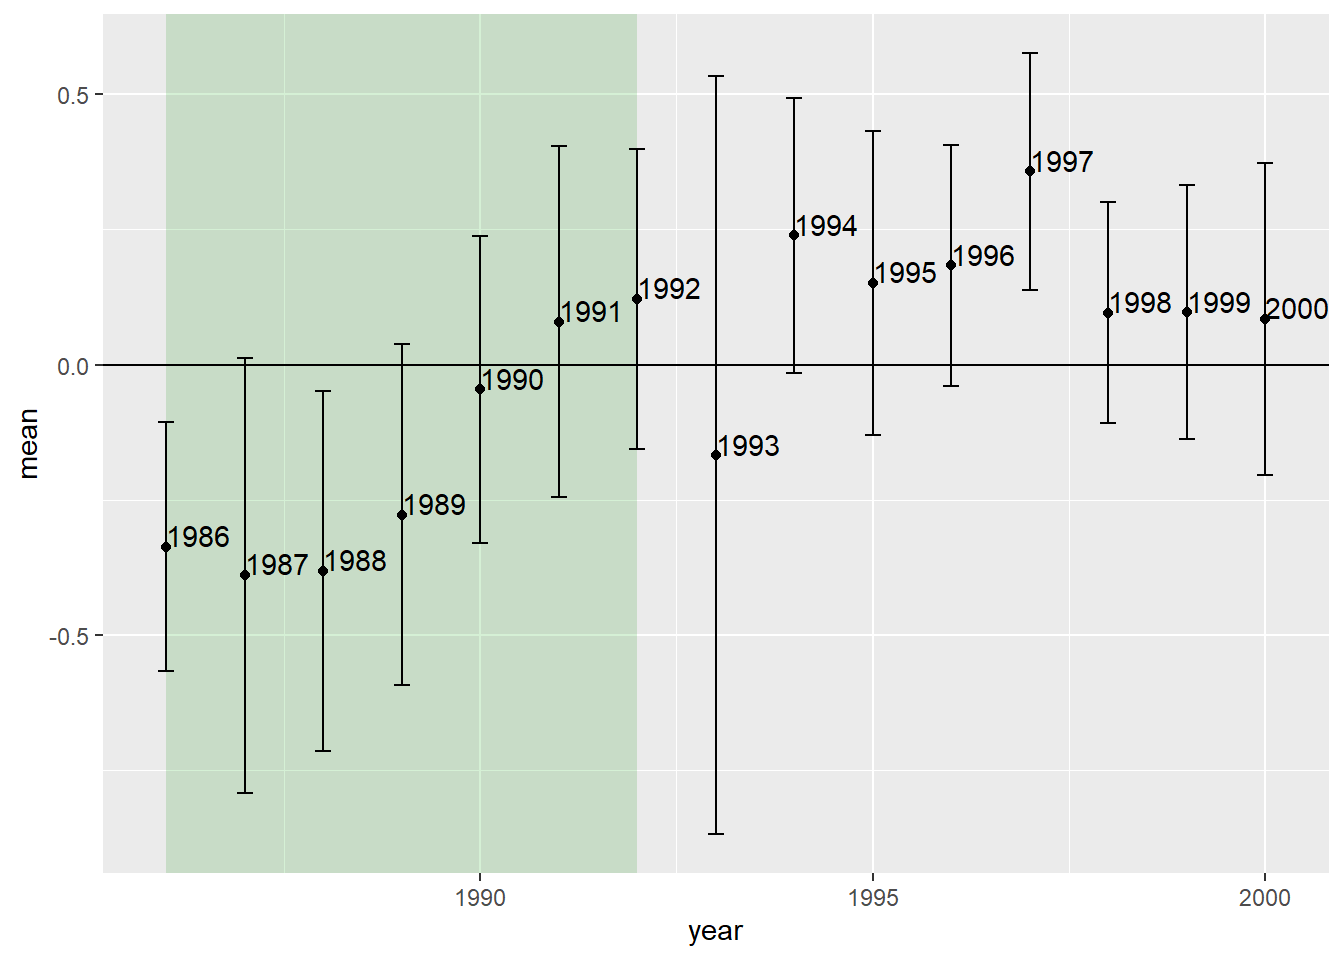
\includegraphics{ReplicacionAbortion_files/figure-latex/unnamed-chunk-2-1.pdf}

\#3

\begin{table}
\centering
\begin{tabular}[t]{lc}
\toprule
  & Model 1\\
\midrule
(Intercept) & \num{7.603}***\\
repeal1 & \num{-1.835}+\\
year1986 & \num{-0.037}\\
year1987 & \num{-0.274}**\\
year1988 & \num{-0.339}***\\
year1989 & \num{-0.396}**\\
year1990 & \num{-0.438}*\\
year1991 & \num{-0.502}**\\
year1992 & \num{-0.763}***\\
year1993 & \num{-0.965}***\\
year1994 & \num{-1.051}***\\
year1995 & \num{-1.350}***\\
year1996 & \num{-1.482}***\\
year1997 & \num{-1.478}***\\
year1998 & \num{-1.418}**\\
year1999 & \num{-1.444}*\\
year2000 & \num{-1.473}*\\
fip4 & \num{-0.668}\\
fip5 & \num{-0.014}\\
fip6 & \num{0.853}+\\
fip8 & \num{-0.764}\\
fip9 & \num{-1.341}+\\
fip10 & \num{-0.829}\\
fip11 & \num{-1.892}\\
fip12 & \num{-0.719}\\
fip13 & \num{-0.502}+\\
fip15 & \num{-0.282}\\
fip16 & \num{-1.635}***\\
fip17 & \num{-0.569}\\
fip18 & \num{-0.144}\\
fip19 & \num{-0.111}\\
fip20 & \num{0.137}\\
fip21 & \num{-0.244}**\\
fip22 & \num{-0.678}*\\
fip23 & \num{-2.146}***\\
fip24 & \num{-1.366}*\\
fip25 & \num{-1.739}*\\
fip26 & \num{-0.694}+\\
fip27 & \num{-0.429}\\
fip28 & \num{-0.015}\\
fip29 & \num{-0.099}\\
fip30 & \num{-1.428}***\\
fip31 & \num{-0.096}\\
fip32 & \num{-1.844}\\
fip33 & \num{-3.525}*\\
fip34 & \num{-2.059}**\\
fip35 & \num{-1.087}***\\
fip36 & \num{-0.174}\\
fip37 & \num{-0.138}\\
fip38 & \num{-2.152}***\\
fip39 & \num{-0.515}*\\
fip40 & \num{0.171}\\
fip41 & \num{-1.087}**\\
fip42 & \num{-0.538}+\\
fip44 & \num{-0.984}+\\
fip45 & \num{-0.963}***\\
fip46 & \num{-1.975}*\\
fip47 & \num{-0.011}\\
fip48 & \num{-0.574}\\
fip49 & \num{-1.914}***\\
fip50 & \num{-2.120}***\\
fip51 & \num{-0.884}*\\
fip53 & \num{0.924}+\\
fip54 & \num{-0.325}\\
fip55 & \num{-0.314}\\
fip56 & \num{-1.657}***\\
acc & \num{0.0009}\\
ir & \num{0.00002}\\
alcohol & \num{0.434}\\
crack & \num{0.071}\\
poverty & \num{0.005}\\
income & \num{0.00004}\\
ur & \num{-0.031}\\
repeal1 × year1986 & \num{-0.091}\\
repeal1 × year1987 & \num{-0.091}\\
repeal1 × year1988 & \num{-0.416}+\\
repeal1 × year1989 & \num{-0.579}**\\
repeal1 × year1990 & \num{-0.555}**\\
repeal1 × year1991 & \num{-0.506}*\\
repeal1 × year1992 & \num{-0.387}*\\
repeal1 × year1993 & \num{-0.240}\\
repeal1 × year1994 & \num{-0.147}\\
repeal1 × year1995 & \num{-0.015}\\
repeal1 × year1996 & \num{-0.102}\\
repeal1 × year1997 & \num{-0.099}\\
repeal1 × year1998 & \num{-0.075}\\
repeal1 × year1999 & \num{-0.024}\\
repeal1 × year2000 & \num{-0.030}\\
\midrule
Num.Obs. & \num{733}\\
R2 & \num{0.849}\\
R2 Adj. & \num{0.829}\\
RMSE & \num{0.35}\\
Std.Errors & by: fip\\
\bottomrule
\end{tabular}
\end{table}

\#4

\begin{table}
\centering
\begin{tabular}[t]{lc}
\toprule
  & Model 1\\
\midrule
(Intercept) & \num{8.434}***\\
repeal1 & \num{-0.588}\\
year1986 & \num{0.005}\\
year1987 & \num{-0.087}\\
year1988 & \num{0.072}\\
year1989 & \num{0.185}\\
year1990 & \num{0.186}\\
year1991 & \num{0.164}\\
year1992 & \num{0.017}\\
year1993 & \num{-0.255}\\
year1994 & \num{-0.067}\\
year1995 & \num{-0.311}\\
year1996 & \num{-0.369}\\
year1997 & \num{-0.320}\\
year1998 & \num{-0.146}\\
year1999 & \num{-0.148}\\
year2000 & \num{-0.188}\\
acc & \num{-0.003}\\
ir & \num{-0.0002}\\
alcohol & \num{0.213}\\
crack & \num{-0.086}\\
poverty & \num{-0.002}\\
income & \num{-0.00003}\\
ur & \num{-0.009}\\
repeal1 × year1986 & \num{0.174}\\
repeal1 × year1987 & \num{0.269}+\\
repeal1 × year1988 & \num{0.051}\\
repeal1 × year1989 & \num{-0.115}\\
repeal1 × year1990 & \num{-0.114}\\
repeal1 × year1991 & \num{-0.150}\\
repeal1 × year1992 & \num{-0.095}\\
repeal1 × year1993 & \num{0.174}\\
repeal1 × year1994 & \num{0.072}\\
repeal1 × year1995 & \num{0.241}\\
repeal1 × year1996 & \num{0.075}\\
repeal1 × year1997 & \num{-0.050}\\
repeal1 × year1998 & \num{-0.033}\\
repeal1 × year1999 & \num{-0.027}\\
repeal1 × year2000 & \num{0.019}\\
\midrule
Num.Obs. & \num{1435}\\
R2 & \num{0.464}\\
R2 Adj. & \num{0.449}\\
RMSE & \num{0.77}\\
Std.Errors & by: fip\\
\bottomrule
\end{tabular}
\end{table}

\end{document}
